\documentclass[11pt,a4paper]{article}
\usepackage[margin=2.3cm]{geometry}
\usepackage{amsmath,amssymb,tikz,hyperref,lmodern}
\usetikzlibrary{decorations.pathreplacing}
\usepackage[T1]{fontenc}
\setlength{\parindent}{0pt}\setlength{\parskip}{6pt}
\newcommand{\code}[1]{\texttt{#1}}
\newcommand{\q}[2]{\medskip\noindent\textbf{Question #1 (#2 points).} }
\begin{document}
\begin{center}{\large CSC\_2F002\_EP --- Design and Analysis of Algorithms}\\[3pt]
{\Large\bfseries Practice Midterm --- Part II}\\[3pt]{\large Finding a majority by random sampling}\end{center}
\textbf{Guidelines.} This part and Part I form one two-hour practice midterm, worth 20 points in total. Complete \code{majority.py}; run \code{python3 test\_majority.py}. Answer the exercise questions in comments at the indicated locations. Tests cannot establish a probability guarantee: your justification must address the algorithm, not just the observed output.

Let \(A\) be a list of \(n\) integers. A value \(x\) is a \emph{strict majority} if it occurs more than \(n/2\) times in \(A\). For example, 5 is a strict majority of \([5,2,5,5,2]\), since it occurs 3 times out of 5. There is no strict majority in \([1,1,2,2]\), since neither value occurs more than half the time. An empty list has no strict majority.

There is at most one strict majority: two distinct values cannot each occupy more than half of the positions. The goal is to find this value, if one exists. We use Python \code{None} to report that no value was found; because the entries are integers, \code{None} is not a possible input value. A randomized procedure may occasionally return \code{None} even when a majority exists, but it must never return a non-majority value.

\q{1}{1} Complete \code{frequency(A, x)} to return the number of occurrences of \code{x} in \code{A}. The function must make a single pass and run in \(O(n)\) time. Return zero when the list is empty.

\q{2}{2} Complete \code{verify(A, x)}. Return \code{x} if it is a strict majority of \code{A}, and return \code{None} otherwise. Run in \(O(n)\) time. For example, \code{verify([0,0,1], 0)} returns 0, not a Boolean. Be careful: 0 is a valid majority, even though \code{bool(0)} is false in Python.

\textbf{Sampling one candidate.} Rather than test all distinct values, choose one \emph{position} uniformly from \(\{0,\ldots,n-1\}\), then test the value at that position. Drawing positions rather than distinct values ensures that a value occurring \(f\) times is sampled with probability \(f/n\). For the example \([5,2,5,5,2]\), 5 is selected with probability \(3/5\).
\newpage
\begin{center}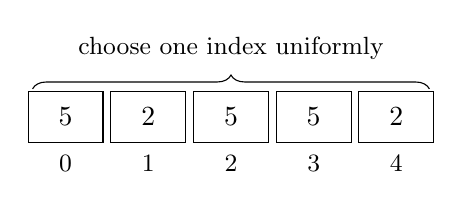
\begin{tikzpicture}[x=1.05cm,y=.65cm]
\foreach \i/\v in {0/5,1/2,2/5,3/5,4/2} {\node[draw,minimum width=.95cm,minimum height=.65cm] at (\i,0) {\v}; \node at (\i,-.9) {\small\i};}
\draw[decorate,decoration={brace,amplitude=5pt}] (-.4,.55)--(4.4,.55);
\node at (2,1.35) {\small choose one index uniformly};
\end{tikzpicture}\\[5pt]\small Figure 1: Indices 0, 2 and 3 select value 5; indices 1 and 4 select value 2.
\end{center}
A call to \code{random.randrange(n)} returns a uniformly random integer from \(0\) to \(n-1\). Assume each call gives a fresh independent uniform draw. The \code{random} module is already imported in the skeleton. Use exactly one call to \code{random.randrange(len(A))} for each trial on a nonempty list. Sampling is with replacement: a position may be drawn again in a later trial.

\q{3}{2} Complete \code{one\_trial(A)}. If \code{A} is nonempty, draw one position as described, verify the value stored at that position, and return the verified value or \code{None}. For an empty list return \code{None} without making a random draw. The result must never be a non-majority. The worst-case running time of one trial must be \(O(n)\).

\textbf{Repeated trials.} We can improve the chance of finding an existing majority by repeating independent trials. Stop immediately if a trial returns a value, and otherwise return \code{None} after \(k\) unsuccessful trials. Since a valid majority may be 0 or a negative integer, test explicitly against \code{None}. If the input has no strict majority, each verification returns \code{None} and the procedure reports \code{None}.

\q{4}{3} Complete \code{find\_majority(A, k)} for an integer \(k\ge0\). Run at most \(k\) independent trials as specified above, stopping as soon as a majority is found. Return \code{None} if \(k=0\) or if \code{A} is empty, without drawing an index. Do not change \code{A}. The worst-case running time must be \(O(kn)\), aside from constant-time handling of empty input and \(k=0\).

For instance, suppose \(A=[5,2,5,5,2]\) and the first two sampled indices are 1 and 3. The first candidate is 2, which fails verification. The second is 5, which passes, so the procedure returns 5 without making a third draw. If all \(k\) sampled positions happen to contain 2, the return value is \code{None}, despite the existence of a majority.
\newpage
\textbf{Analyzing the probability.} Suppose a strict majority occurs at \(f\) of the \(n>0\) positions. The probability of drawing it on any one trial is \(f/n>1/2\). Each trial samples independently with replacement. Verification guarantees that a returned integer is a genuine strict majority; an error can only be a failure to find an existing one.

\q{5}{2} In the comment block marked \code{Q5} in \code{majority.py}, answer the following. (a) Express the exact probability that \code{find\_majority(A,k)} returns \code{None} when the majority has frequency \(f\). Explain why the draws can be multiplied. (b) Give a simple upper bound on this probability depending only on \(k\). (c) Give a sufficient integer \(k\) to make the failure probability at most \(1/1000\), and justify the choice. Also explain briefly why the procedure cannot return a wrong integer. Include the case \(k=0\) in your formula.

\textbf{A note on testing random algorithms.} The tests replace the random number generator with predetermined indices so that successes, failures and early stopping are reproducible. This checks the implementation for those sequences; it does not prove independence or the probability bound. In normal use the skeleton calls Python's \code{random.randrange}. You may run the tests more than once; they should give the same results.

\textbf{Additional checks.} A one-element list has a strict majority. A list of even length with two values appearing exactly half the time has none. For \code{[0,0,1]} a verified 0 must be returned immediately, not confused with failure. None of the functions should modify the input list.
\end{document}
